\begin{blocksection}
\question Let the path sum of any node in the tree be equal to the sum of its label and the labels of all nodes on the path from the root to that node. For example, for the following tree:
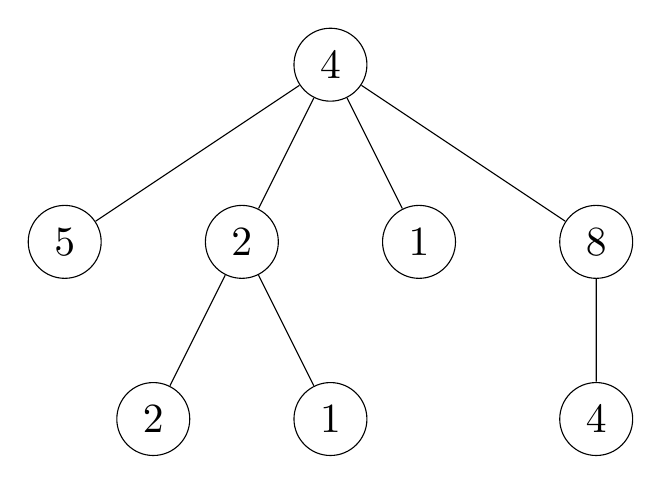
\begin{tikzpicture}[scale=1.5, transform shape]
    \node [circle, draw] (z){$4$}
        child {node [circle, draw] (a) {$5$}}
        child {node [circle, draw] (b) {$2$}
            child {node [circle, draw] (e) {$2$}}
            child {node [circle, draw] (f) {$1$}}
        }
        child {node [circle, draw] (c) {$1$}}
        child {node [circle, draw] (d) {$8$}
            child {node [circle, draw] (g) {$4$}}
        };
\end{tikzpicture}

The path sum of each node in the tree is as follows:

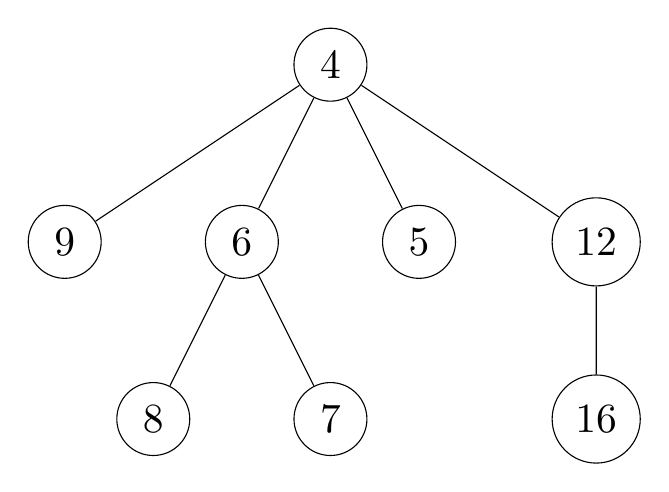
\begin{tikzpicture}[scale=1.5, transform shape]
    \node [circle, draw] (z){$4$}
        child {node [circle, draw] (a) {$9$}}
        child {node [circle, draw] (b) {$6$}
            child {node [circle, draw] (e) {$8$}}
            child {node [circle, draw] (f) {$7$}}
        }
        child {node [circle, draw] (c) {$5$}}
        child {node [circle, draw] (d) {$12$}
            child {node [circle, draw] (g) {$16$}}
        };
\end{tikzpicture}

Write a generator that takes in a Tree object and yields the path sum of each node in the tree. The path sum of a node should be yielded only after the path sum of all of its children have been yielded. (Tangential note: this ordering is called post-order DFS). See doctests.


\begin{lstlisting}
def gen_path_sums(t):
    """
    >>> t = Tree(1, [Tree(2, [Tree(5)]), Tree(3, [Tree(4)])])
    >>> print(list(gen_path_sums(t)))
       	[8, 3, 8, 4, 1] # draw out the tree and check your understanding!
    >>> 
    """    
    for _____________________________
    	for _______________________________
    		_______________________________
    _______________________
\end{lstlisting}
\end{blocksection}

\begin{blocksection}
\begin{solution}[0.5in]
\begin{lstlisting}
def gen_path_sums(t):
    for b in t.branches:
        for branch_sum in gen_path_sums(b):
            yield t.label + branch_sum
    yield t.label
\end{lstlisting}
Typically, when we solve problems with trees, we want to solve them using recursion because recursion works very naturally with trees since every branch of a tree is a tree itself.  Since we want to go through the paths in order, setting up a \lstinline{for b in t.branches} loop is a good start.  Now what do we want to do for each branch is yield all paths that are a part of that branch. This is a good place to use recursion, since what we want here are the path sums of each branch.  However, remember that calling a generator function always evaluates to a generator object, so we can’t just \lstinline{yield gen_paths_sum(b)}. What we need to do instead is yield each value from the generator object returned from \lstinline{gen_paths_sum(b)}, which we can do by iterating through the values of \lstinline{gen_paths_sum(b)} by using a for loop \lstinline{(for paths_sum in gen_paths_sum(b))}. Then the last thing we need to remember is that we need to add the label to each path yielded from \lstinline{gen_paths_sum(b)}. 

Note that we do not just want to yield the sums of all the paths from the root to a leaf but rather we want to yield the sums of all of the paths from the root to each node in the tree (including the path from the root to itself) regardless of if that node is a leaf or not. Therefore, after we have yielded all of the values of the current lable + the sum of the paths in the branches, we also want to yield just the current label itself which will be used to construct the sum from the root to this label and not any of the labels in its branches.
\end{solution}
\end{blocksection}
